\chapter{基于深度卷积网络的线虫前景轮廓提取}
\section{引言}
秀丽隐杆线虫由于通体透明,且PDMS制作的微流控芯片也是透明的,所以线虫轮廓的分割是个难点。
通过简单的阈值分割的方法,并不能够很好的分割线虫的轮廓,因为前景像素的灰度值范围被包括在背景像素的灰度范围内。
通过背景减除的方法分割的线虫轮廓。由于图像噪声的影响,会导致分割的线虫轮廓出现断裂、不完整等情况。
这些都会导致线虫跟踪的失败。另一方面,背景的估计需要$50\sim100$帧背景不变的图像。
当需要对线虫进行实时跟踪时,基于背景估计的线虫前景分割算法需要一个启动时间用于背景的估计。
另外,当CCD相机或载物台移动时(如:需要观察不同腔室中的虫子),由于背景的改变,这种算法还是会失效。
卷积网络作为一种强大的特征提取器在许多计算机视觉中取得了很大的成功。

	本课题将卷积网络用于线虫轮廓的前景提取具有如下优势:
	
\begin{enumerate}
  \item 与基于背景减除的方法相比,基于卷积网络的分割不需要对图像背景建模,只依赖当前帧的图像,从而能够保证实时性的要求。
  \item 能够降低硬件成本,传统的线虫图像处理,为了获得一个背景和线虫轮廓对比度比较高的图像。通常使用特制的硬件对CCD和照明都有很高的要求。卷积网络作为一种强大特征提取器降低了对图像质量的要求。
  \item 鲁棒性更好,传统的线虫轮廓分割算法,通常需要人工的选取一些超参数(如:分割的阈值,形态学操作中核的大小等等),但由于视频采集过程中照明的变化以及图像噪声的影响很难选取一个最佳的全局参数。
基于卷积网络的分割是一种端到端的方法,输出直接是分割的结果,因此,这种方法不依赖超参数的选取,具有很好的鲁棒性。
\end{enumerate}
\section{线虫图像处理总体方案介绍}
	线虫图像处理的总体流程如图\ref{fig:flow}所示,共分成4个阶段。第一个阶段是从采集到的视频中读取一帧图像,并将
	线虫轮廓覆盖的区域定义为前景,剩下的区域视为背景。这一阶段的输出为一幅二值化的图像,其中1表示前景0表示
	背景。如果是单线虫的跟踪,则第一个阶段的输出则为线虫的轮廓。但考虑到多线虫跟踪过程中多个线虫的轮廓会出现
	相交甚至纠缠在一起,导致因无法区分单个线虫从而跟踪丢失。第二个阶段的任务主要是对多个线虫相交的轮廓进行解析,
	从而得到单个线虫的轮廓。第三个阶段的线虫跟踪是利用线虫轮廓的重心面积等信息找出相邻两帧图像之间线虫轮廓的对应
	关系。第四个阶段主要是利用跟踪到的线虫轮廓计算出线虫体长、运动速度等信息。本章主要介绍线虫图像处理流程中
	第一个阶段的内容。

	\begin{figure}[h]
	  \centering
	  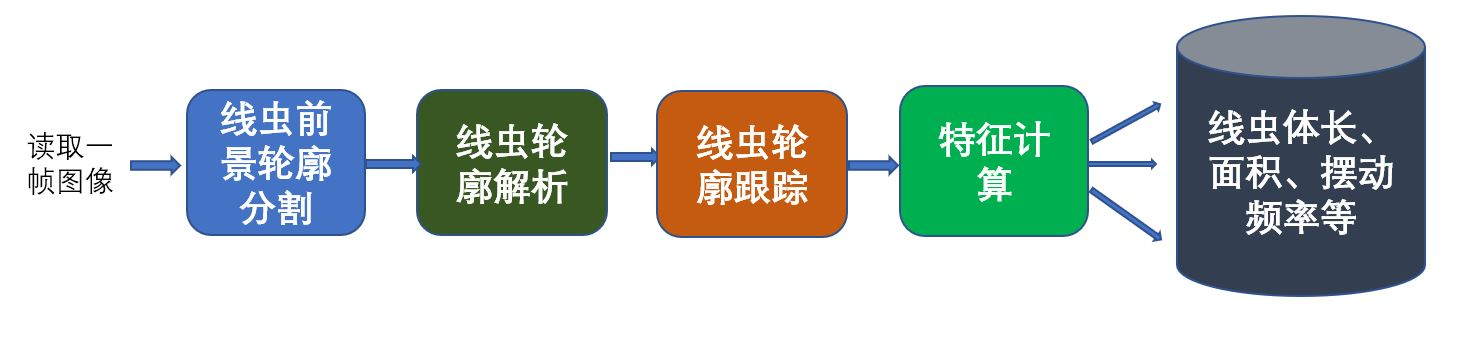
\includegraphics[width=14cm]{figure/chap3/flow.jpg}
	  % \hspace{1cm}
	  % 
\includegraphics[width=4cm]{example/sjtulogo.jpg}
	  \bicaption[这里将出现在插图索引中]
		{线虫图像处理总体流程图}
		{The flow chart of C.elegans image processing}
	  \label{fig:flow}
	\end{figure}
\section{传统的图像分割方法分类介绍}
	图像分割是生物医疗图像处理任务最重要的步骤之一,图像分割指的是将图像按照预先定义的
	相似度准则将图像划分为若干个区域的过程,相似度准则可以是代表同一个对象的像素
	的特性或特征。
\subsection{基于像素的图像分割方法}
	基于像素的阈值分割方法通过利用图像灰度直方图的统计信息来确定一个或者多个阈值来,
	并对图像中每个像素进行比较和分类。其中OSTU于1979年提出了基于最大类间方差的阈值分割方法,
	通过最大化类间方差计算出一个全局最优阈值。与全局阈值法相对应的是自适应阈值的分割,由于每个像素的阈值
	是根据其局部邻域内的统计直方图计算的,所以对于光照不均匀的图像其具有很好的分割效果。除了以上提到
	的两种方法外,还有最大熵阈值法、双峰法、P参数法等。
	
	与通过阈值将像素分为多个类别的阈值分割方法不同,基于像素聚类的分割是通过对像素的灰度值或者特征
	向量的聚类实现图像分割。如彩色图像往往具有R、G、B三个通道,因此可以将每个像素的三个颜色通道的
	分量值添加到该像素的特征向量里。这是像素聚类的一个优势,其能够利用每个像素更多的信息,而阈值分割
	只能利用像素的灰度值。像素聚类往往产生不连续带有孔洞的区域或者具有单个孤立像素的区域,所以聚类后
	一般都需要后处理算法以消除这些缺陷。常用的后处理算法有区域生长、像素连接和一些基于规则的算法等。
	常见的聚类算法有K均值聚类算法和以模糊集合为基础的Fuzzy cmeans(FCM)聚类聚类算法等。
\subsection{基于边缘的图像分割方法}
	基于边界的图像分割方法通常使用空间滤波的方法计算图像的一阶梯度和二阶梯度。Sobel算子常被用于
	计算图像的一阶梯度信息。Laplacian算子常被用于计算图像的二阶梯度信息。使用这些微分算子对图像进行空间滤波
	便可以将图像中不同区域的边缘检测出来。由于图像中噪声的影响,这些边缘通常是不连续的。
	为了形成闭合的区域,通常需要将这些不连续的边连接起来。常用的算法有Canny边缘检测算法。
\subsection{基于区域的图像分割方法}
	基于区域生长的图像分割方法是根据预先定义的相似性准则将相邻的像素或或或相邻的区域融合形成一个
	大的区域。当原图像被过度分割成很多小区域时,区域生长的方法作为一种有效的后处理方法能够处理分割
	过程中目标轮廓出现断裂的情况。与区域生长相对应的是区域分裂,这种方法可以将一个大的区域分割成两个
	或者更多的小区域。另外,区域分裂的分割方法可能使目标轮廓产生孔洞。
\subsection{交互式的图像分割方法}
	所谓交互式的图像分割方法指的是需要用户提供输入的分割方法(如:需要用户提供一个矩形框或者鼠标点击
	等输入操作),是一种半自动化的图像分割方法。目前常见的交互式图像分割方法有基于图论的GrabCut算法\cite{rother2004grabcut}
	和基于曲线演化的活动轮廓分割方法。GrabCut算法是由Rother等人于2004年提出,通过引入Gibbs能量函数,将前景背景分割
	问题转化为一个能量最小化的问题,通过迭代计算的方式将能量最小化。在分割的过程中,用户还用画刷将某个区域标记为前景或
	背景,然后让算法继续迭代以改善分割的性能。另一方面,基于活动轮廓的分割方法总是能够获得连续的闭合的轮廓。
	特别是将水平集理论应用于活动轮廓分割使得该方法可以自动处理轮廓的分裂和合并,使其更具灵活性。其原理
	是曲线在某些力的作用下呈现扩张或者收缩的运动,最终会收敛于目标轮廓的边缘。但是活动轮廓的分割方法需要
	提供一个初始轮廓作为算法的输入,因此也是一种半自动化的分割方法。
\subsection{基于背景减除的分割方法}

\section{线虫轮廓前景分割卷积网络的设计及模型评估}

\subsection{数据集的制作}
\subsubsection{数据集的采集}
	图\ref{fig:chap5:camera}是线虫图像采集的系统装置图,主要由显微镜、CCD相机、照明系统和微流控芯片四个部分组成,CCD
	相机通过数据线连接电脑进行图像数据传输。线虫通过注射泵注入到微流控芯片的腔室内。移动显微镜的载物台使线虫腔室
	位于视野的正中央。调节显微镜的放大倍数使线虫腔室充满整个视野。调整显微镜焦距使视野中呈现清晰的图像。调整CCD相机的
	曝光时间以获得一个对比度比较高的线虫图像。完成以上步骤后便可以进行线虫视频的录制。
	\begin{figure}[thb]
	  \centering
	  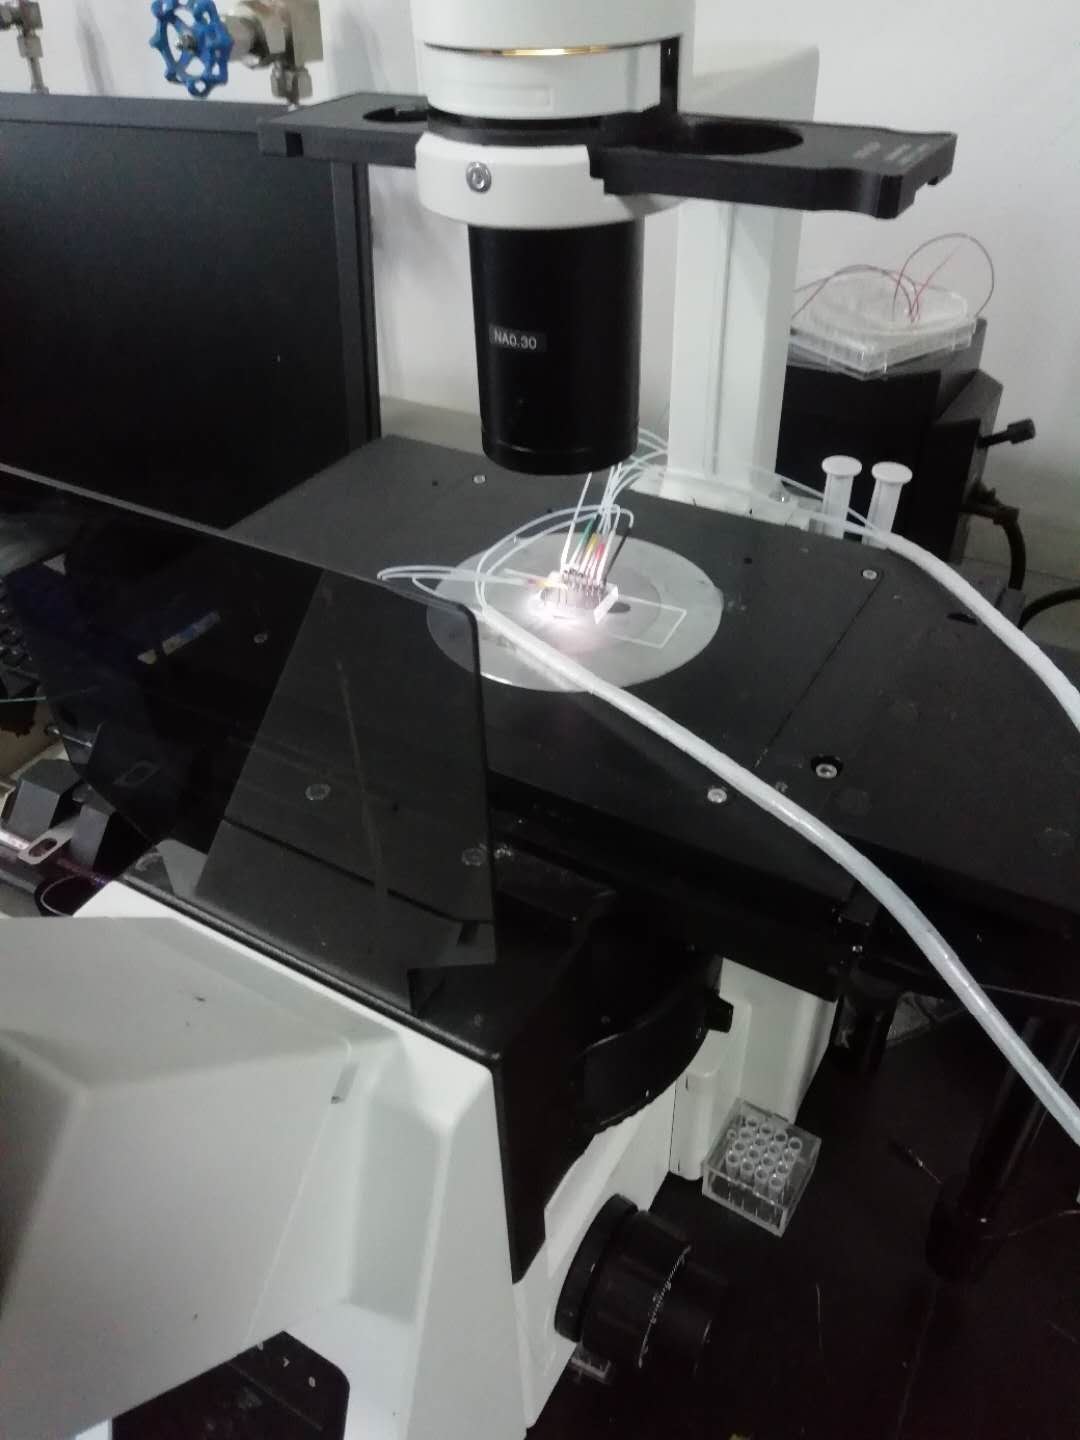
\includegraphics[width=8cm]{figure/chap5/camera.jpg}
	  \bicaption[这里将出现在插图索引中]
		{图像采集系统图}
		{Change in contour curvature}
	  \label{fig:chap5:camera}
	\end{figure}
\subsubsection{数据集的标注}
	高质量的数据集对网络的训练来说至关重要,且数据集的质量决定了神经网络模型性能的上限,通过优化网络架构的方法
	也只能逼近这个上限。但数据集的标注通常是一个非常耗时的过程,特别是图像分割任务要对不同的区域标记。目前很多的
	图像分割的标注工具(如:Labelme\footnote{\url{https://github.com/wkentaro/labelme}}和Ratesnake\footnote{\url{https://is-innovation.eu/ratsnake/}}等)都是采用多边形近似的标注方法,
	即在轮廓的四周边缘采集足够多的点,这些点构成的多边形为标注对象的轮廓。由于线虫形态变化复杂,相对于其他目标
	的标注往往需要采集更加密集的点才能满足线虫轮廓标注的精度。为了提高线虫图像标注的效率,本文采用了一种半自动的线虫轮廓
	标注方法。将Grabcut算法用于线虫轮廓的标注,只需要用矩形框将线虫轮廓框出作为Grabcut算法输入,算法可以自动的分割
	出线虫的轮廓,最后再将多个线虫轮廓合成为一个标签图像。通过这种方法,本文制作了一个包含211个样本的数据集,图\ref{fig:dataset}是数据集部分示例。
	整个数据集按照$8:2$的比例将数据集分为训练集与测试集两部分分别用于网络模型的训练与测试。
	\begin{figure}[h]
	  \centering
	  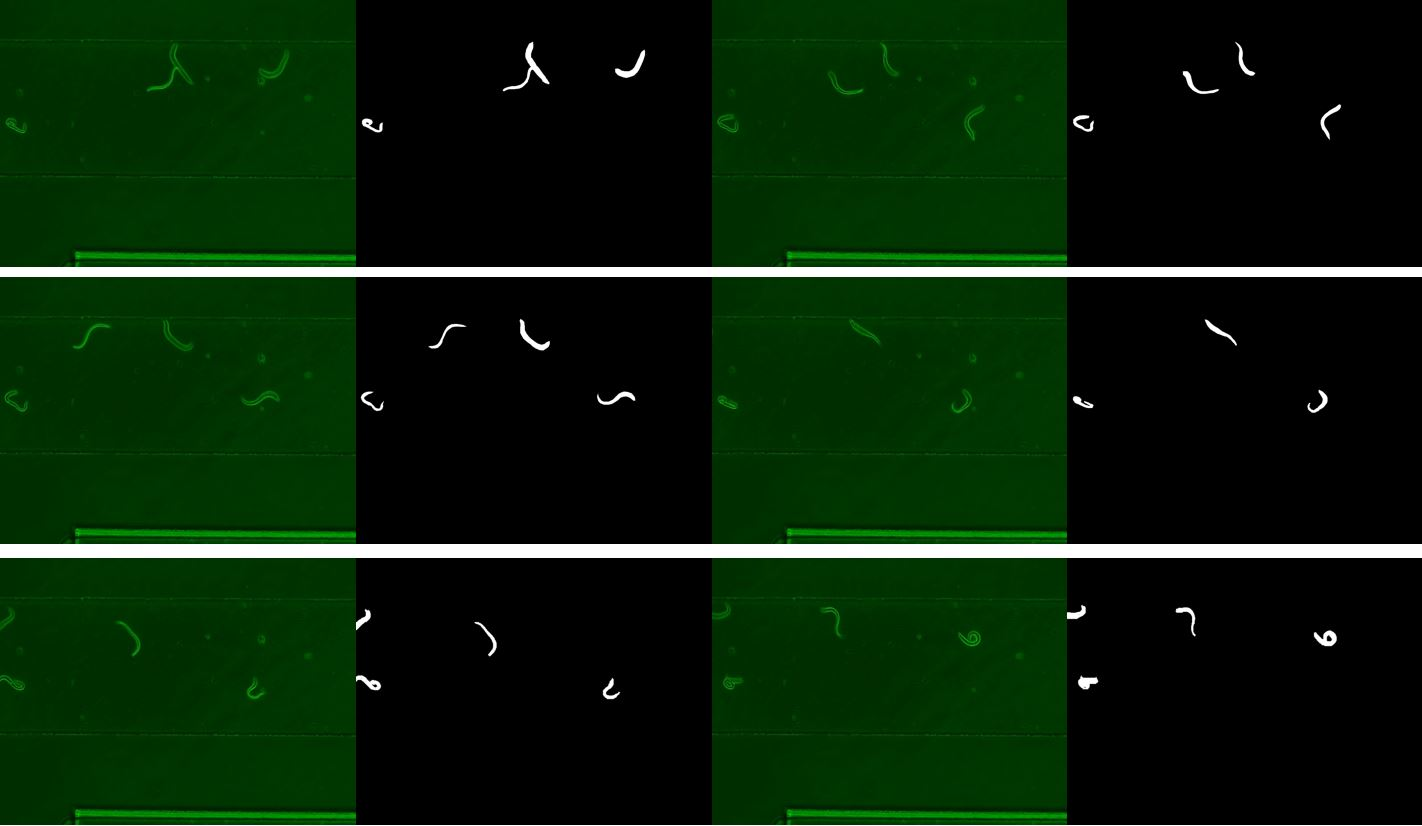
\includegraphics[width=14cm]{figure/chap3/dataset.jpg}
	  % \hspace{1cm}
	  % 
\includegraphics[width=4cm]{example/sjtulogo.jpg}
	  \bicaption[这里将出现在插图索引中]
		{数据集示例}
		{The flow chart of C.elegans image processing}
	  \label{fig:dataset}
	\end{figure}
\subsection{条件随机场模型在分割任务中的应用}
	
\subsection{网络结构的设计}

\subsection{网络模型的训练}

\subsection{实验结果分析}

\section{本章小结}